\section{Evaluation}
Giza provides fault tolerance through erasure coding across wide area networks while providing linearizability for its read and write operations. As such, there are currently no system that is specifically designed to serve as an alternative to Giza. However, we benchmark Giza’s performance against Cassandra and CockroachDB to illustrate the following points:

- In the common case, Giza’s Fast Paxos implementation of the metadata phase allows for lower latency writes for Giza when compared to Cassandra.

- While one could implement Giza’s metadata phase and data phase as a single distributed transaction, we illustrate through CockroachDB that doing so will degrade performance significantly.

In addition, we provide evaluation results for encoding scheme ranging from 2-1 in 3 data centers to 18-4 in 22 data centers to illustrate the flexibility of Giza as a front end.
\subsection{Setup}
For our experiments, we deploy a single azure virtual machine (16 cores, 56 GB of RAM, 800 GB SSD, and gigabit ethernet) and set up a local storage account for each data center. For each storage account, we deploy a Blob storage and a Table storage and set the replication level for both to locally redundant. Each virtual machine runs a giza node and can serve requests from the users. Since we only tolerate a single data center failure, the number of giza nodes participating in the metadata phase is fixed at 3 for the classical paxos implementation and 4 for the fast paxos implementation. If the data path involves sending more than 3 or 4 data fragments, this set of Giza node is a subset of the total number of Giza nodes with the other Giza nodes only serving data path requests.The role of the Giza nodes in each data center and how many is determined by the clients per our use case.

To set up CockroachDB, we use the same azure virtual machine instances and run a single CockroachDB node. We followed the recommended production settings by the developers of CockroachDB when deploying these instances. For example, on the same virtual machine, we also run NTP to provide moderately accurate time to preserve data consistency. Other optimizations can be found on the CockroachDB website. We only benchmark CockraochDB against Giza in the 3 dc cluster scenario since we want the fault tolerance level to be the same for the comparisons.
Since variability in latency is a factor when benchmarking cloud storage, we run all our experiments at approximately the same time.
Since latency is an issue, we run all our experiments at around the same time.
We experimented with different erasure coding schemes
For all experiments, we deployed a single virtual machine (16 cores, 56 GB of RAM, 800 GB SSD, and gigabit ethernet) for each geographical region. We use the same virtual machines for setting up the Cassandra and CockroachDB clusters. The client issuing the requests runs on one of the virtual machine that is also part of the cluster. 
To set up Giza, we also had to deployed both a table service and a blob service provided by the cloud service platform. The granularity of replication for these services varies from provider to provider but we always choose the replication level to match that of the regional replication. This means that as long as there’s no dc outage, the data would not be lost. For each data center, we run a Giza node frontend with the virtual machine. The Giza node can service requests from a client running in the virtual machine. In addition, requests to its local table and blob storage from other Giza nodes also go through the Giza node frontend in the form of an RPC call. This is to avoid unecessary WAN round trips when dealing with complicated table and blob storage operations. 

How did we set up Cassandra?

This is how we set up Cassandra.

How did we set up CockroachDB?

We run a CockroachDB cluster spanning all the data centers included in the experiment where each node correspond to the virtual machine running on each geographical region. We use a single database of CockroachDB to emulate our Giza read and write path. The database contains multiple tables, a metadata table and multiple data tables corresponding to their respective region, and the tables differ in their replication level. The metadata table is replicated according to the fault tolerance level, i.e 2 if the the cluster can tolerate one data center outage [what about the location?]. The data table is replicated once only at the node of the respective region.
*machines*

We generate our workloads using the YCSB benchmark. Since our systems function as key value blob storage, we only require one field, the blob value, for each key. The probability that a given key will be accessed is given by the Zipfian distribution. We evaluated our systems with different blob value sizes. The smaller sizes include 64KB, 128KB, 256KB, and 512 KB while the bigger sizes include 1MB, 2MB, 4MB, and 8MB. We also evaluated them under different read/write ratios, including equal-shares and all writes.

\subsection{Giza Read/Write Latency}
We measure Giza's latency performance by running 1000 write and read operations with a single threaded Giza node.We vary the object size (1mb and 4mb) and compared different configurations. 
The 95th percentile latency result is shown in Figure 4. The four configurations we chose are 3 data centers in the US (2-1 erasure coding scheme), 3 data centers across the world, 7 data centers in the US (6-1 erasure coding scheme), and 7 data centers across the world. Both the configuration (i.e distance between data centers) and the size of the object impact latency peformance. Larger objects incur higher latency in both the vm to vm transfer and the local blob storage access. This can explain the similar put latency results between the 3 US data center configuration and the 7 US data center configuration. Even though in the 3 US data center configuration, the distance between the data centers are much shorter (Iowa, Illinois, and West Central), each data fragment is 2MB. We can see in Table 3 that this increases the latency performance for the data path. In the 7 US data center configuration, each data fragment is just 700 KB, which reduces latency even when the data centers are further away. 

% \begin{figure}[!h]
% \centering
%   \subfloat[Giza Put 99th Percentile]{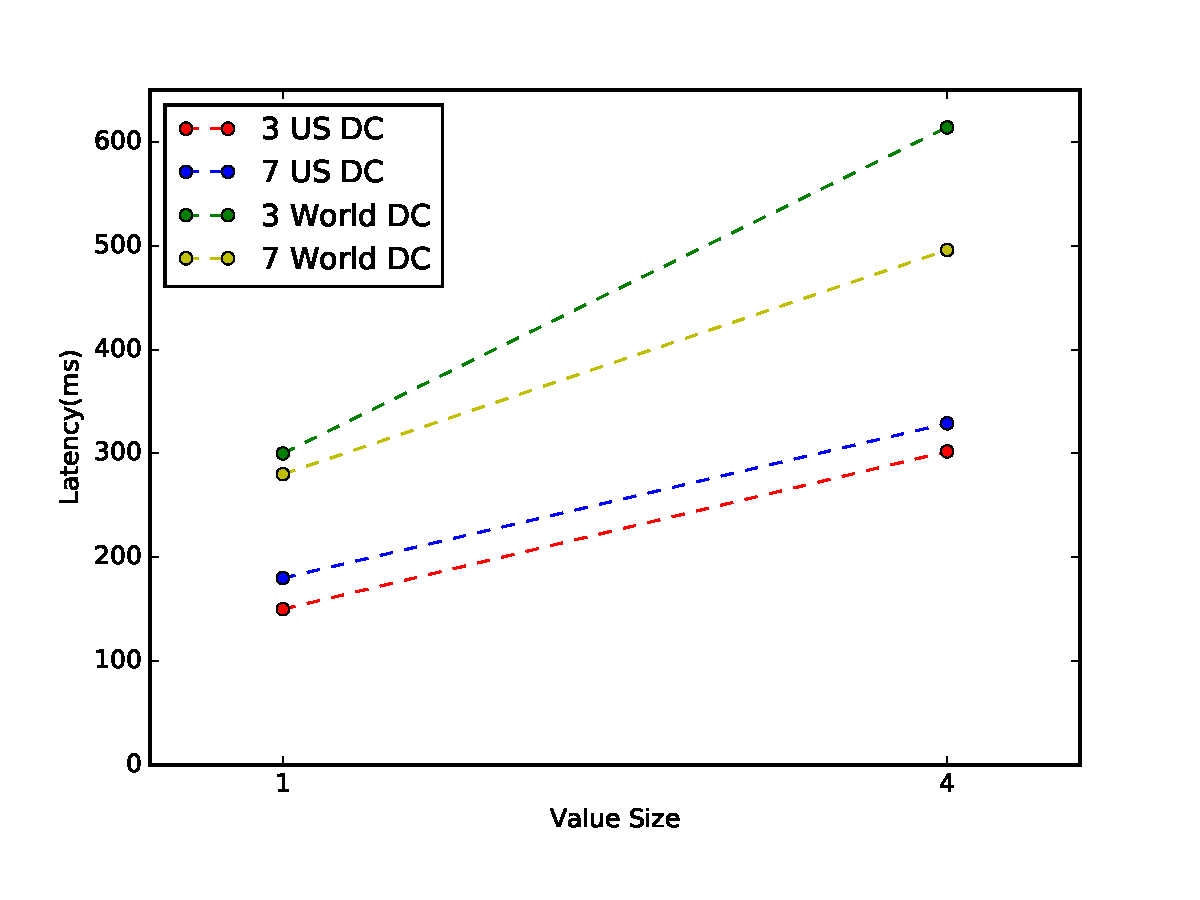
\includegraphics[width=0.5\textwidth]{images/write_latency}\label{fig:f1}}
%   \subfloat[Giza Get 99th Percentile]{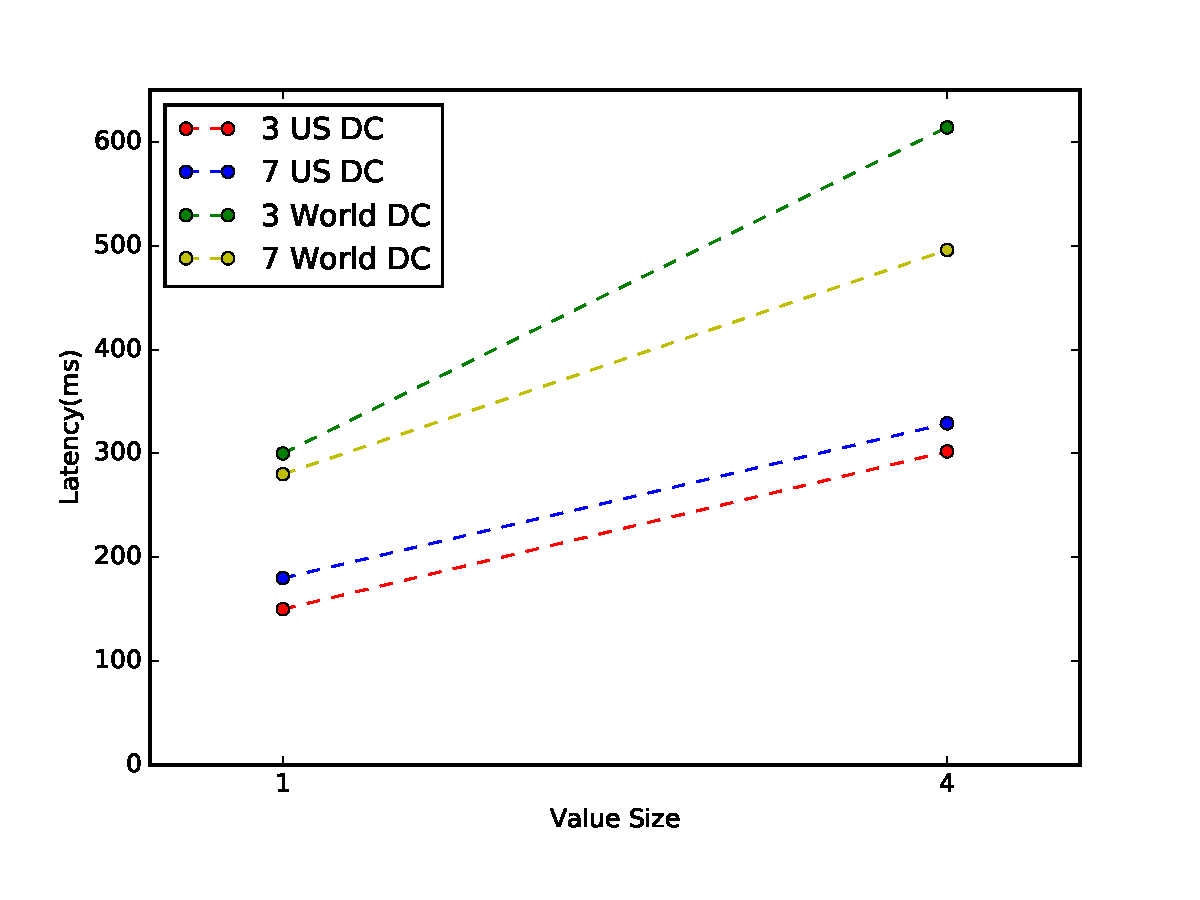
\includegraphics[width=0.5\textwidth]{images/write_latency}\label{fig:f2}}
% \caption{Comparison of latency of the four configurations}
% \end{figure}

\subsection{Comparing Giza with CockroachDB}
We benchmark the performance of Giza with CockroachDB in two cases. In the first case, we use CockroachDB as a geo-replicating blah blah blah. Here is the result.
In the second case, we used cockroachdb's transaction to simulate what we are doing with Giza. Blah blah blah, here is the result.
64K $\sim$ 16MB

X-axis: Value size
Y-axis: 50\% Read latency

X-axis: Value size
Y-axis: 90\% Read latency

X-axis: Value size
Y-axis: 99\% Read latency

Same for write

[adding cpu results in a table]

\subsection{Large object}
256MB $\sim$ 1GB

X-axis: Value size
Y-axis: Average Read latency

X-axis: Value size
Y-axis: Average Write latency


\subsection{Contention}

Fixed object size
X-axis: zipf coefficient
Y-axis: 50\%, 90\%, 99\% Read/Write Latency


\subsection{Real workload}
Table.